\section{Diagramas de Clase}

Los diagramas de clases están ordenados por importancia y bloque funcional, siguiendo una
perspectiva bottom-up siempre que sea posible.


\subsubsection{Clase MM.Class}
Como centro de todo el sistema de clases implementado está el MM.Class. Una abstracción del 
patrón constructor que es eje de todas las clases implementadas en la aplicación. A partir 
de ahora, cuando hable de clase me refiero a la herencia efectuada con MM.Class.

La implementación de este objeto es fundamental ya que Javascript es un lenguaje orientado 
a objetos puro y libre de clases. 

\begin{figure}[tbph]
\centering
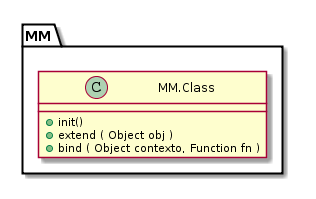
\includegraphics[width=0.4\linewidth]{imagenes/diagrama-clase-mm-class}
\caption{Clase MM.Class}
\label{fig:diagrama-clase-mm-class}
\end{figure}
Los principales métodos son:   
\begin{itemize}
\item \textbf{MM.Class.extend:} método que nos permite extender sobre una clase existente.
\item \textbf{MM.Class.init:} Constructor para las clases.
\end{itemize}

Cualquier método sobrescrito dispone en su clase una propiedad \underline{ }super que hace referencia al método sobrescrito, de forma
podamos realizar una llamada al super (o padre).


\subsection{Diagrama de clases PubSub}

Como núcleo en la comunicación, entre clases y distintos bloques funcionales, están los eventos. Para ello, se ha desarrollado
la clase MM.PubSub que implementa el patrón Publicador-Suscriptor\footnote{También conocido como patrón Observador-observable}.

\begin{figure}[tbph]
\centering
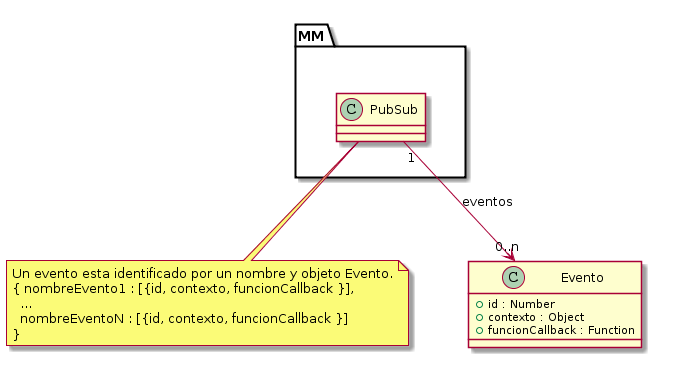
\includegraphics[width=\linewidth]{imagenes/diagrama-clases-mm-pubsub}
\caption{Diagrama de clases pubsub}
\label{fig:diagrama-clases-mm-pubsub}
\end{figure}


El concepto es sencillo, el objeto suscriptor se suscribe a un evento o mensaje concreto y el publicador anuncia a todos los 
suscriptores cuando está lista las suscripción. El símil más utilizado, y directo, es el de los suscriptores de un periódico, 
el cual un lector (o suscriptor) paga un precio para recibir el periódico y la editorial (o publicador) le envía un ejemplar 
cuando lo tiene disponible. 


Los eventos suscritos se registran con un nombre en una lista, que contiene un identificador de suscripción, el contexto de 
ejecución y la función a ejecutar en el momento de la publicación del evento.

\subsubsection{MM.PubSub}
\begin{figure}[tbph]
\centering
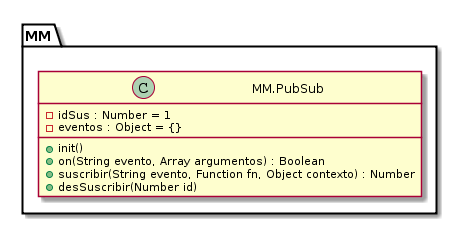
\includegraphics[width=0.5\linewidth]{imagenes/diagrama-clase-mm-pubsub}
\caption{Clase MM.PubSub}
\label{fig:diagrama-clase-mm-pubsub}
\end{figure}

Métodos:
\begin{itemize}
\item \textbf{MM.PubSub.suscribir:} permite a los suscriptores la suscripción a un evento o publicación.
\item \textbf{MM.PubSub.desSuscribir:} permite a los suscriptores la de suscripción a un evento o publicación.
\item \textbf{MM.PubSub.on:} método que permite al publicador notificar a los suscriptores
la ocurrencia de un evento. 
\end{itemize}





\subsection{Diagrama de clases MM.UndoManager}

Dentro de la edición, otro punto importante son las funciones de hacer y deshacer. Para ello, se ha implementado un manejador que se encarga de registrar, en una lista de comandos, los cambios 
realizados en el editor.

\begin{figure}[tbph]
\centering
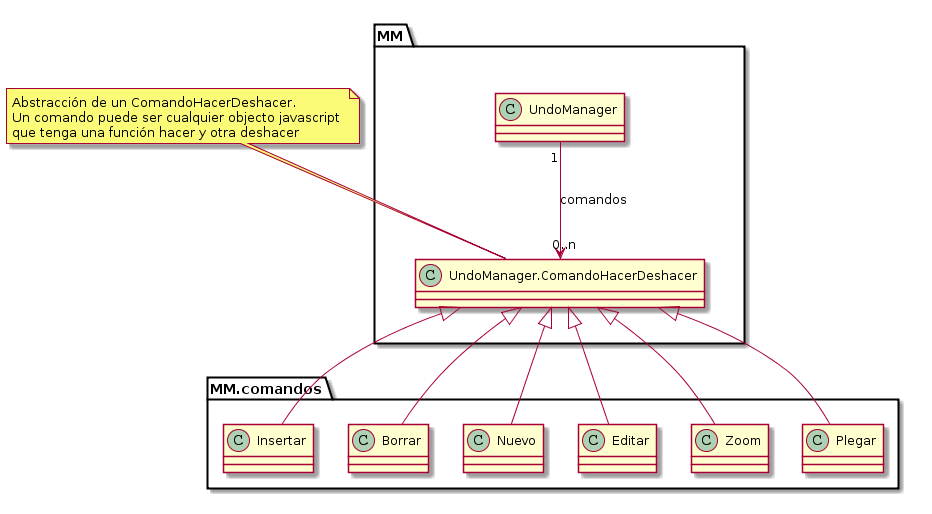
\includegraphics[width=\linewidth]{imagenes/diagrama-clases-mm-undo}
\caption{Diagrama de clases undo}
\label{fig:diagrama-clases-mm-undo}
\end{figure}

\subsubsection{Clase MM.UndoManager.ComandoHacerDeshacer}

La clase MM.UndoMangerComandoHacerDeshacer es la clase base para todos los comandos para hacer y
deshacer del editor de mapas mentales. De ella, como se puede observar en la figura \ref{fig:diagrama-clases-mm-undo}, heredan clases para hacer y deshacer inserciones, borrados, 
zoom, etc ...  

\begin{figure}[tbph]
\centering
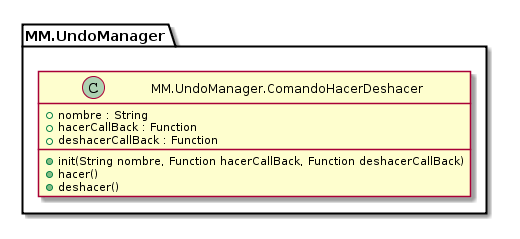
\includegraphics[width=0.7\linewidth]{imagenes/diagrama-clase-mm-undomanager-comandohacerdeshacer}
\caption{Clase MM.UndoManager.ComandoHacerDeshacer}
\label{fig:diagrama-clase-mm-undomanager-comandohacerdeshacer}
\end{figure}

Todo comando deberá tener un nombre e implementar los métodos hacer y deshacer. La funcionalidad del 
método hacer se encargará de repetir la operación ejecutada y el deshacer de revertirla.

\subsubsection{Clase MM.UndoManager}

El manejador de acciones hacer/deshacer tiene un registro de comandos ejecutados en la aplicación y un puntero\footnote{Campo actual.} que indica el último comando ejecutado. El comportamiento es que siempre se puede deshacer la última acción ejecutada, apuntada por actual, y sólo se puede hacer el comando siguiente al puntero actual.

\begin{figure}[tbph]
\centering
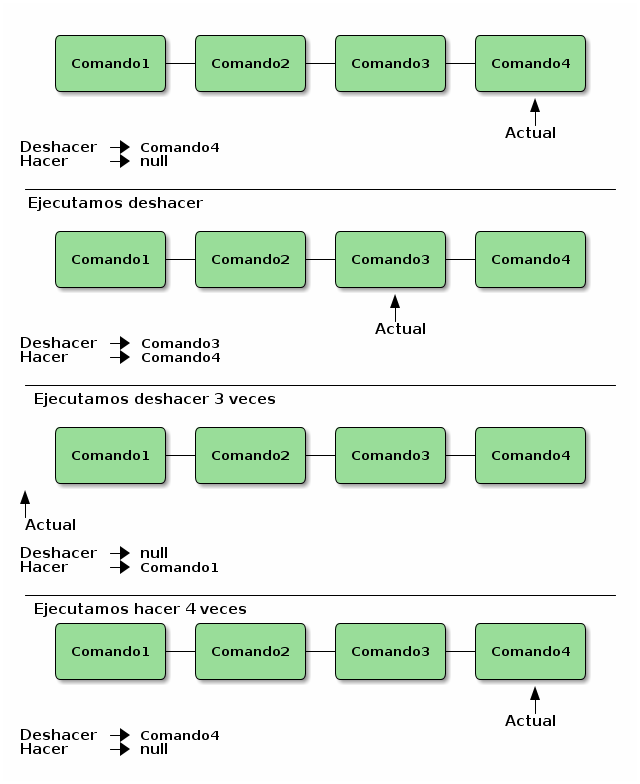
\includegraphics[width=0.7\linewidth]{imagenes/undomangerEjecucion.png}
\caption{Secuencia de ejecución de UndoManager}
\label{fig:undomanager-ejecucion}
\end{figure}
 
Como puede observar en la figura \ref{fig:undomanager-ejecucion} el puntero \textit{Actual} indica que comando se puede deshacer y \textit{Actual + 1} el comando que se puede hacer. 

\begin{figure}[tbph]
\centering
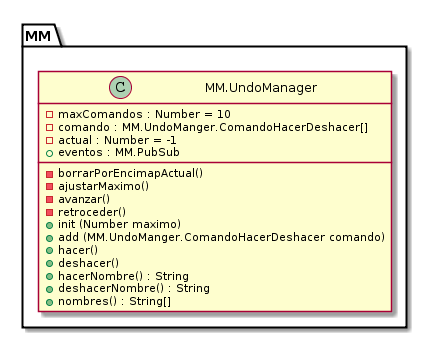
\includegraphics[width=0.7\linewidth]{imagenes/diagrama-clase-mm-undomanager}
\caption{Clase MM.UndoManager}
\label{fig:diagrama-clase-mm-undomanager}
\end{figure}

Los métodos:
\begin{itemize}
\item \textbf{MM.UndoManager.init:} al constructor se le puede indicar el máximo de la pila 
de ejecución.
\item \textbf{MM.UndoManager.add:} añade un nuevo comando a la pila de ejecución.
\item \textbf{MM.UndoManager.hacer:} ejecuta el hacer del comando que apunta actual + 1 y avanza 
el puntero. 
\item \textbf{MM.UndoManager.deshacer:} ejecuta el deshacer del comando que apunta actual y 
retrocede el puntero.
\item \textbf{MM.UndoManager.hacerNombre:} devuelve el nombre del siguiente comando hacer.
\item \textbf{MM.UndoManager.deshacerNombre:} devuelve el nombre del siguiente comando deshacer.
\item \textbf{MM.UndoManager.nombres:} lista de comandos en la lista.
\end{itemize}






\subsection{Diagrama de clases MM}

El centro de la aplicación es sin lugar a dudas el módulo MM. El módulo MM aglutina y vertebra la 
ejecución del editor de mapas mentales. 

\begin{figure}[tbph]
\centering
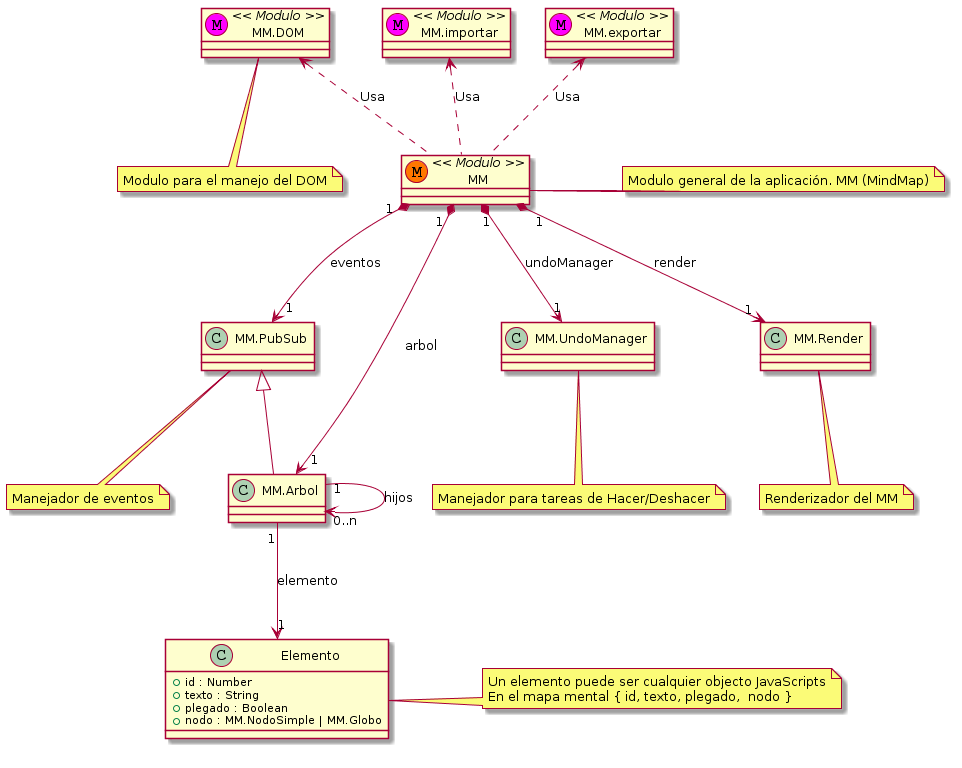
\includegraphics[width=\linewidth]{imagenes/diagrama-clases-mm}
\caption{Diagrama de clases MM}
\label{fig:diagrama-clases-mm}
\end{figure}

Una mapa Mental (MM) tiene un árbol que representa la estructura del mapa mental y un manejador de 
eventos con el que podemos publicar los eventos de la aplicación para avisar a otras partes integrantes del sistema\footnote{Por ejemplo al render o al interface de usuario}. Así pues cuando el usuario añade un añade un nuevo elemento al mapa mental, MM se encargará:

\begin{itemize}
\item Mantener la coherencia de los datos.
\item Registrar el comando ejecutado en el UndoManager
\item Y avisar o publicar el evento de para indicar la operación realizada.
\end{itemize}

Cada elemento de un nodo del árbol tiene un id de nodo, un texto, un indicador de plegado y un nodo gráfico.

\subsubsection{Módulo MM}

\begin{figure}[tbph]
\centering
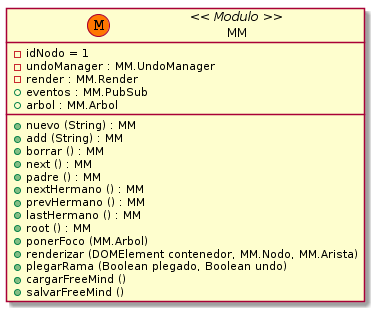
\includegraphics[width=0.5\linewidth]{imagenes/diagrama-clase-mm}
\caption{Clase MM}
\label{fig:diagrama-clase-mm}
\end{figure}

El módulo tiene los siguientes métodos:
\begin{itemize}
\item \textbf{MM.nuevo:} crea un nuevo mapa mental.
\item \textbf{MM.add:} añade un nuevo nodo hijo al nodo activo.
\item \textbf{MM.borrar:} borra el nodo activo.
\item \textbf{MM.next:} mueve el foco al primer hijo del nodo activo.
\item \textbf{MM.padre:} mueve el foco al padre del nodo activo.
\item \textbf{MM.nextHermano:} mueve el foco al siguiente hermano del nodo activo.
\item \textbf{MM.prevHermano:} mueve el foco al hermano anterior del nodo activo.
\item \textbf{MM.lastHermano:} mueve el foco al último hermano del nodo activo.
\item \textbf{MM.root:} mueve el foco al nodo raíz.
\item \textbf{MM.ponerFoco:} establece el foco en nodo dado.
\item \textbf{MM.renderizar:} se encarga de renderizar el mapa mental.
\item \textbf{MM.plegarRama:} función para plegar y desplegar ramas.
\item \textbf{MM.cargarFreeMind:} función de carga de ficheros FreeMind.
\item \textbf{MM.salvarFreeMind:} se encarga de salvar el mapa mental en formato FreeMind.
\end{itemize}



\subsubsection{Clase MM.Arbol}

\begin{figure}[tbph]
\centering
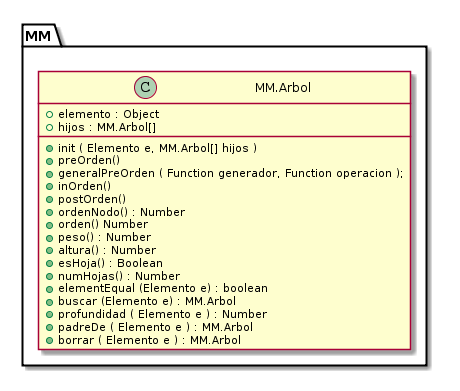
\includegraphics[width=0.7\linewidth]{imagenes/diagrama-clase-mm-arbol}
\caption{Clase MM.Arbol}
\label{fig:diagrama-clase-mm-arbol}
\end{figure}

La implementación MM.Arbol debe ser una implementación funcional de un árbol-n lo más general posible. 

\begin{itemize}
\item \textbf{MM.Arbol.init:} Crea un nuevo árbol-n con un elemento raíz y array de árboles hijos.
\item \textbf{MM.Arbol.preOrden:} realiza un recorrido en preorden por el árbol.
\item \textbf{MM.Arbol.generalPreOrden:} recorrido en preorden, con un generador que trata el elemento actual y una operación que se encarga de operar el elemento generado con el preorden de los nodos hijos.
\item \textbf{MM.Arbol.inOrden:} realiza un recorrido inorden por los elementos del árbol.
\item \textbf{MM.Arbol.postOrden:} recorre el árbol el postorden.
\item \textbf{MM.Arbol.ordenNodo:} calcula el orden del nodo actual.
\item \textbf{MM.Arbol.orden:} calcula el orden del árbol completo.
\item \textbf{MM.Arbol.peso:} calcula el peso de un árbol.
\item \textbf{MM.Arbol.altura:} altura del árbol.
\item \textbf{MM.Arbol.esHoja:} indica si el nodo actual es un nodo hoja o no.
\item \textbf{MM.Arbol.numHojas:} determina el número de nodos hojas del árbol.
\item \textbf{MM.Arbol.elementEqual:} función de igual entre elementos de los nodos. Por defecto, es la igual estricta "===". Esta función podrá ser sobreescrita para adecuarse al tipo de elemento guardado en cada nodo.
\item \textbf{MM.Arbol.buscar:} busca un elemento en el árbol. Como comparador de nodos se utiliza la función MM.Arbol.elementEqual.
\item \textbf{MM.Arbol.profundidad:} determina la profundidad del árbol.
\item \textbf{MM.Arbol.padreDe:} calcula el árbol padre del elemento pasado.
\item \textbf{MM.Arbol.borrar:} borra un elemento del árbol.
\end{itemize}



\subsubsection{Módulo MM.DOM}

El módulo MM.DOM contendrá funciones para el manejo del DOM. Creación y borrado de elementos DOM. 

\begin{figure}[tbph]
\centering
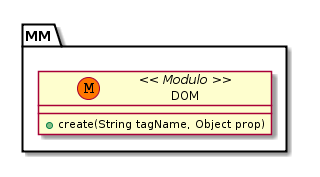
\includegraphics[width=0.4\linewidth]{imagenes/diagrama-clase-mm-dom}
\caption{Modulo MM.DOM}

\label{fig:diagrama-clase-mm-dom}
\end{figure}



\subsubsection{Clase MM.Render}

La clase MM.Render es la encargada de pintar el mapa mental y realizar los ajustes visuales necesarios para mostrar los nodos y las aristas. El renderizador se configura o inicializa entorno a un elemento DOM, normalmente un \textit{div}, una clase que MM.NodoSimple\footnote{O que herede de MM.NodoSimple como MM.Globo} y una clase MM.Arista\footnote{O que herede de MM.Arista}. A partir de estos datos el sistema es capaz de ir generando el mapa mental en función de los eventos producidos en el módulo MM. 

\begin{figure}[tbph]
\centering
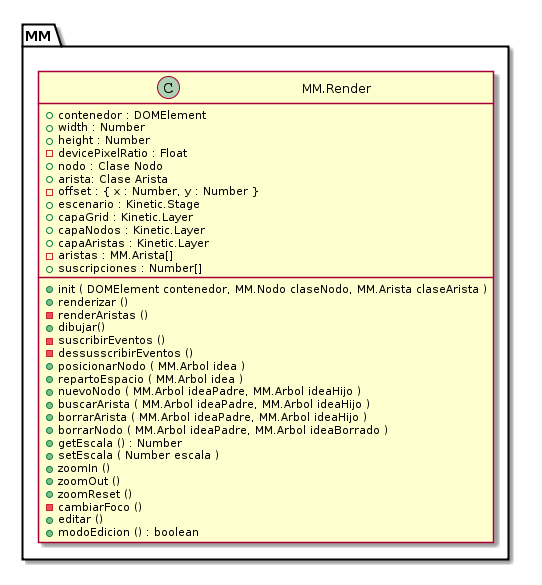
\includegraphics[width=0.65\linewidth]{imagenes/diagrama-clase-mm-render}
\caption{Modulo MM.Render}

\label{fig:diagrama-clase-mm-render}
\end{figure}

La clase MM.Render dispone de los siguientes métodos: 
\begin{itemize}
\item \textbf{MM.Render.init:} constructor de la clase render. Inicializas las capas del de nodos y aristas. 
\item \textbf{MM.Render.renderizar:} se encarga de realizar las suscripciones a eventos, dibujar y establecer los atajos de teclado.
\item \textbf{MM.Render.renderizarAristas:} pinta las aristas entre los distintos nodos.
\item \textbf{MM.Render.dibubar:} en función del mapa actual del módulo MM dibuja y reparte el espacio de dibujo.
\item \textbf{MM.Render.suscribirEventos / dessuscribirEventos:} métodos de activar y desactivar las suscripciones a eventos del render.  
\item \textbf{MM.Render.get/setEscala:} establece o devuelve la escala actual.
\item \textbf{MM.Render.zoomIn / zoomOut / zoomReset :} funciones de zoom, en orden, aumenta, disminuye o reinicia la escala del mapa mental.
\item \textbf{MM.Render.cambiarFoco:} se encarga de resalta la idea que tiene el foco actual.
\item \textbf{MM.Render.modoEdicion:} indica si la idea actual esta en modo de edición o no.
\item \textbf{MM.Render.editar:} establece la idea actual en modo de edición. Mostrando el editor del nodo y activando y desactivando atajos de teclados y eventos.
\item \textbf{MM.Render.nuevoNodo:} manejador de eventos para cuando se inserta una nueva idea. Se encarga de insertar la nueva idea y enlazar la idea padre con la hija mediante una arista. El sistema de establece la mejor ubicación para el nuevo elemento.
\item \textbf{MM.Render.borrarNodo:} manejador de eventos para cuando se borra un idea y la correspondiente arista. Además se debe redistribuir el mapa mental en función de los nodos restantes.
\item \textbf{MM.Render.buscarArista:} busca una arista entre dos ideas.
\item \textbf{MM.Render.borrarArista:} borra una arista existente entre dos ideas.
\end{itemize}



\subsection{Diagrama de clases nodo.}
El nodo se encarga del pintado de una idea del mapa mental, en esencia, es un MM.Mensaje al cual se le han añadido otros elementos gráficos y funcionalidades. Existen dos implementaciones de nodo, como se pueden ver en el diagrama\ref{fig:diagrama-clases-mm-render}, el MM.NodoSimple y el MM.Globo, y ambos pueden ser usados desde MM.Render. Todos los nodos existen un escenario y en una capa dada. 

\begin{figure}[tbph]
\centering
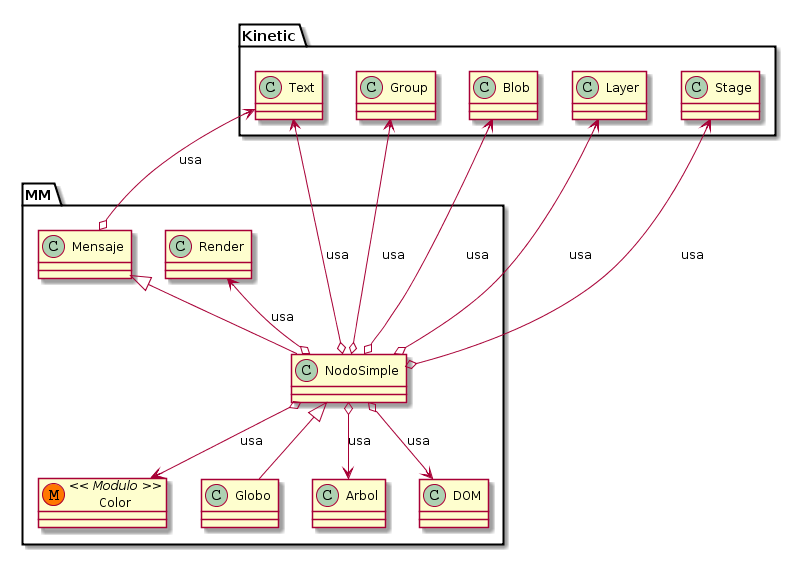
\includegraphics[width=\linewidth]{imagenes/diagrama-clases-mm-render}
\caption{Diagrama de clases nodo}
\label{fig:diagrama-clases-mm-render}
\end{figure}


\subsubsection{Clase MM.Mensaje.}
Se trata de una simple clase que pinta un texto en una capa dada. 

\begin{figure}[tbph]
\centering
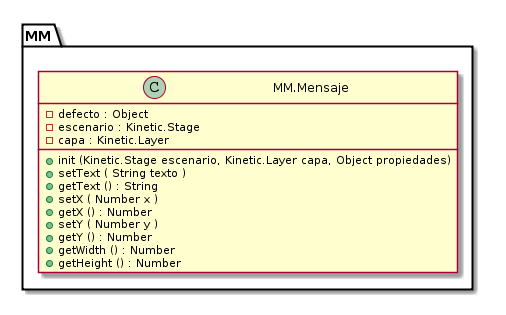
\includegraphics[width=0.7\linewidth]{imagenes/diagrama-clase-mm-mensaje}
\caption{Clase MM.Mensaje}
\label{fig:diagrama-clase-mm-mensaje}
\end{figure}

\begin{itemize}
\item \textbf{MM.Mensaje.init:} constructor de la clase. Tiene el escenario y la capa donde pintar el mensaje, además de un objeto de propiedades con la posición, texto, etc...
\item \textbf{MM.Mensaje.getText/setText:} métodos para establecer y obtener el texto del mensaje. 
\item \textbf{MM.Mensaje.getX/setX:} métodos para establecer y obtener la posición\footnote{en píxeles} X del mensaje.
\item \textbf{MM.Mensaje.getY/setY:} métodos para establecer y obtener la posición Y\footnote{en píxeles} del mensaje.
\item \textbf{MM.Mensaje.getWidth:} devuelve el ancho del texto en píxeles.
\item \textbf{MM.Mensaje.getHeight:} devuelve el alto del texto en píxeles.
\end{itemize}

\subsubsection{Clase MM.NodoSimple.}
Hereda de MM.Mensaje y representa un mensaje o idea subrayado. El nodo representa una idea que será renderizado y creado desde MM.Render. Su funcionalidad básica pasa por obtener el foco cuando sea la idea activa, poderse editar, ocultar cuando su rama este plegada o mostrar cuando este desplegada.

\begin{figure}[tbph]
\centering
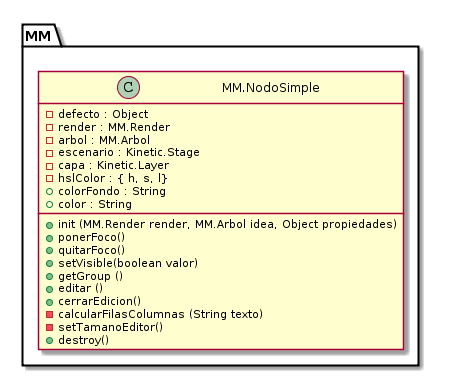
\includegraphics[width=0.6\linewidth]{imagenes/diagrama-clase-mm-nodosimple}
\caption{Clase MM.NodoSimple}
\label{fig:diagrama-clase-mm-nodosimple}
\end{figure}

\begin{figure}[tbph]
\centering
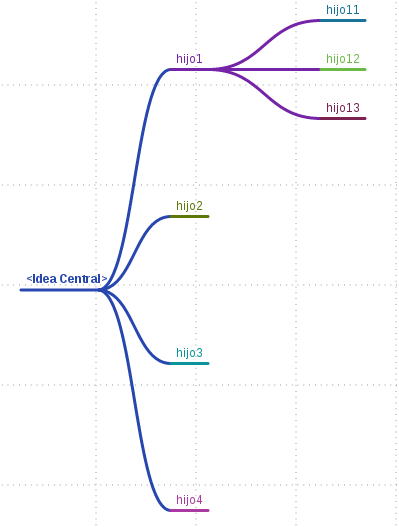
\includegraphics[width=0.5\linewidth]{imagenes/NodoSimple}
\caption{Mapa mental con renderización de nodos simples}
\label{fig:nodosimple}
\end{figure}

\begin{itemize}
\item \textbf{MM.NodoSimple.init:} constructor de la clase. Recibe el MM.Render, la idea a la que representa y un conjunto de propiedades como la posición, escala, etc ...
\item \textbf{MM.ponerFoco/quitarFoco:} métodos que poner o quitan el foco en la idea que representa el nodo. Debe resaltar el nodo cuando este esté focalizado. 
\item \textbf{MM.Mensaje.editar/cerrarEdicion:} métodos para establecer la idea en modo edición y para cerrarlo cuando se termine la edición. Si esta en modo edición debe tener el foco.
\item \textbf{MM.Mensaje.setVisible:} indica si el mensaje debe mostrarse o no.
\item \textbf{MM.Mensaje.destroy:} borra y destruye el nodo.
\end{itemize}


\subsubsection{Clase MM.Globo.}
Se trata de un nodo más elaborado. Representa al texto de la idea incluido en un globo.

\begin{figure}[tbph]
\centering
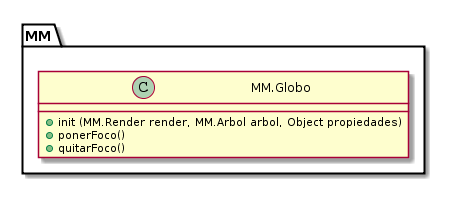
\includegraphics[width=0.6\linewidth]{imagenes/diagrama-clase-mm-globo}
\caption{Clase MM.Globo}
\label{fig:diagrama-clase-mm-globo}
\end{figure}

\begin{figure}[tbph]
\centering
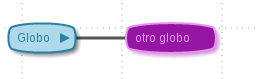
\includegraphics[width=0.3\linewidth]{imagenes/NodoGlobo}
\caption{Mapa mental con renderización de nodos globo}
\label{fig:nodoglobo}
\end{figure}

\subsubsection{Módulo MM.Color.}
Módulo con funcionalidades de color. Permite generar distintos representaciones de color\footnote{HSL, RGB y HUE} y realizar conversiones sobre los distintos tipos. 

\begin{figure}[tbph]
\centering
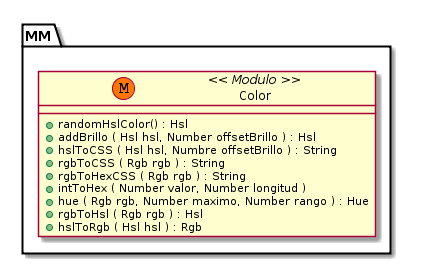
\includegraphics[width=0.5\linewidth]{imagenes/diagrama-clase-mm-color}
\caption{Modulo MM.Color}
\label{fig:diagrama-clase-mm-color}
\end{figure}



\subsection{Diagrama de clases de aristas.}
Una arista representa la línea de unión entre dos ideas o nodos. Existen dos tipos de aristas MM.Arista y MM.Rama, ambas tienen dos nodos a los deben unir. Las aristas, han sido implementadas con una curva Beizer. El diagrama de clases de aristas podemos ver lo en la figura \ref{fig:diagrama-clases-mm-aristas}.

\begin{figure}[tbph]
\centering
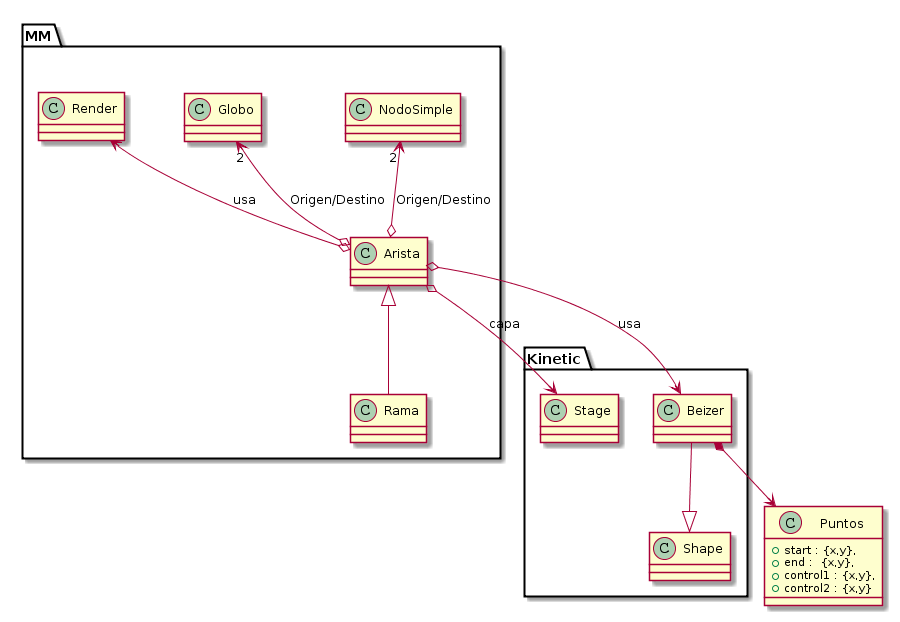
\includegraphics[width=\linewidth]{imagenes/diagrama-clases-mm-aristas}
\caption{Diagrama de clases aristas}
\label{fig:diagrama-clases-mm-aristas}
\end{figure}

\subsection{Clase Kinetic.Beizer.}
Extensión realizada en la librería KineticJS. Una curva Beizer está representada por cuatro puntos inicio, fin y dos puntos de control que determinan la curvatura. En el constructor debe recibir un objeto con los puntos de inicio, fin y de control. Esta clase se encarga de pintar en un canvas la curva en cuestión. 

\begin{figure}[tbph]
\centering
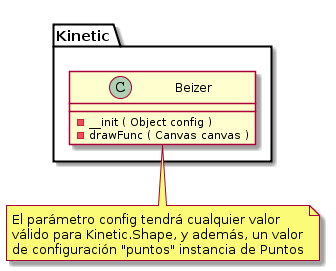
\includegraphics[width=0.5\linewidth]{imagenes/diagrama-clase-kinetic-beizer}
\caption{Clase Kinetic Beizer}
\label{fig:diagrama-clase-kinetic-beizer}
\end{figure}

\subsubsection{Clase MM.Arista.}
Una arista recibe dos ideas y un tamaño (o grosor de línea). Esta clase en cuestión se encarga de unir dos ideas mediante una curva beizer, y de mantenerlos unidos a pesar de los cambios.

\begin{figure}[tbph]
\centering
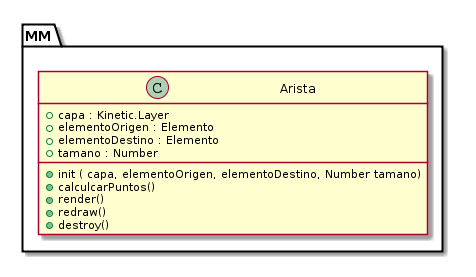
\includegraphics[width=0.7\linewidth]{imagenes/diagrama-clase-mm-arista}
\caption{Clase MM.Arista}
\label{fig:diagrama-clase-mm-arista}
\end{figure}

\begin{itemize}
\item \textbf{MM.Arista.init:} constructor de la clase.
\item \textbf{MM.Arista.calcularPuntos:} calcula los puntos para dibujar la curva.
\item \textbf{MM.Arista.render:} dibuja la curva beizer.
\item \textbf{MM.Arista.rendraw:} redibuja la curva beizer para adaptarse a los cambios producidos en su entorno.
\item \textbf{MM.Arista.destroy:} borra y destruye la arista.
\end{itemize}


\subsubsection{Clase MM.Rama.}
Se trata de otro tipo de arista pensada para unir dos nodos de tipo MM.NodoSimple.

\begin{figure}[tbph]
\centering
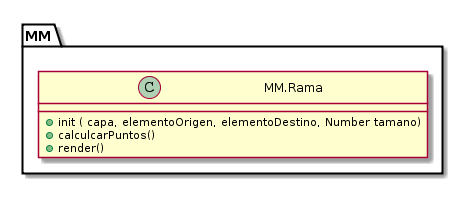
\includegraphics[width=0.7\linewidth]{imagenes/diagrama-clase-mm-rama}
\caption{Clase MM.Rama}
\label{fig:diagrama-clase-mm-rama}
\end{figure}



\subsection{Diagrama de clases de teclado}
Para una mejor experiencia de usuario se ha implementado un complejo manejador de teclados para procesar teclas del tipo \textit{Modificadores+tecla}. El manejo de teclado en el mundo web puede complicarse bastante ya que dependen del navegador y el sistema operativo, ya no sólo por que pueden existir o no teclas como \textit{Meta}\footnote{En los sistemas Mac.} o \textit{Windows}, si no por que existen teclas como \textit{+} que tienen distinto keycode en un Firefox, Chrome y Safari.

También hay que tener en cuenta que las aplicaciones webs no han sido pensadas para un uso intensivo de teclado.   

\begin{figure}[tbph]
\centering
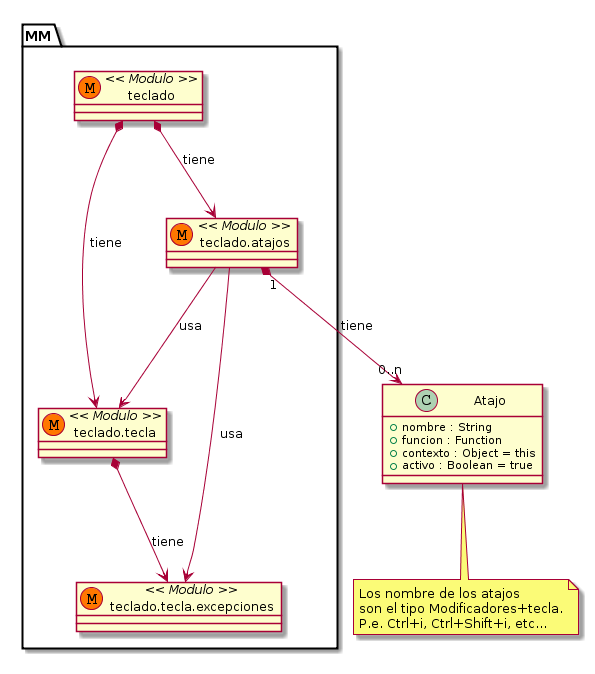
\includegraphics[width=0.8\linewidth]{imagenes/diagrama-clases-mm-teclado}
\caption{Diagrama de clases teclado}
\label{fig:diagrama-clases-mm-teclado}
\end{figure}


\subsubsection{Módulo MM.teclado.atajos}
Un atajo esta compuesto por un nombre\footnote{Ctrl+i}, una función que será ejecutada cuando se
detecte la pulsación de la secuencia de teclas. Un atajo puede estar activado o desactivado, es
decir, que se ejecutará cuando se detecte el atajo de teclado o no. 

El modulo de atajos registrar los atajos de teclados del sistema.


\begin{figure}[tbph]
\centering
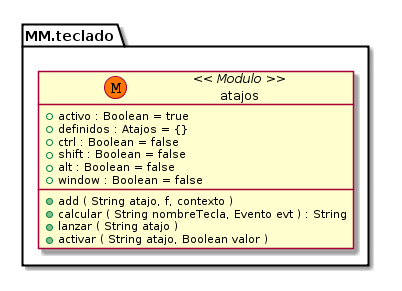
\includegraphics[width=0.6\linewidth]{imagenes/diagrama-clase-mm-teclado-atajos}
\caption{Modulo MM.teclado.atajos}
\label{fig:diagrama-clase-mm-teclado-atajos}
\end{figure}

\begin{itemize}
\item \textbf{MM.teclado.atajos.add:} añade un nuevo atajo de teclado al sistema.
\item \textbf{MM.teclado.atajos.calcular:} calcula el atajo de teclado producido.
\item \textbf{MM.teclado.atajos.lanzar:} lanza un atajo de teclado, es decir, la función asociada. 
\item \textbf{MM.teclado.atajos.activar:} activa o desactiva un atajo de teclado 
\end{itemize}

\subsubsection{Módulo MM.teclado.tecla}
Se trata de un conjunto de constantes de códigos de teclados. También incluye las posibles
excepciones y discordancias que se producen entre los distintos navegadores y sistemas operativos.

\begin{figure}[tbph]
\centering
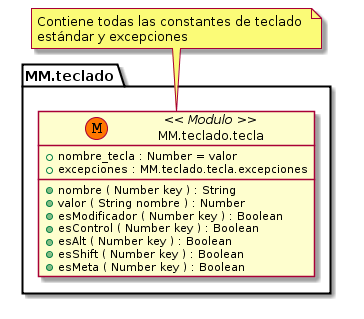
\includegraphics[width=0.4\linewidth]{imagenes/diagrama-clase-mm-teclado-tecla}
\caption{Clase MM.teclado.tecla}
\label{fig:diagrama-clase-mm-teclado-tecla}
\end{figure}

\begin{itemize}
\item \textbf{MM.teclado.tecla.nombre:} calcula el nombre de una tecla en función de su código.
\item \textbf{MM.teclado.tecla.valor:} nos devuelve el código de tecla en función del nombre.
\item \textbf{MM.teclado.tecla.esModificador:} indica si un código de teclado es un modificador. 
\item \textbf{MM.teclado.tecla.esControl:} indica si el código de teclado se corresponde con la tecla $<$Control$>$.
\item \textbf{MM.teclado.tecla.esAlt:} indica si el código de teclado se corresponde con la tecla $<$Alt$>$.
\item \textbf{MM.teclado.tecla.esShift:} indica si el código de teclado se corresponde con la tecla $<$Shift$>$.
\item \textbf{MM.teclado.tecla.esMeta:} indica si el código de teclado se corresponde con la tecla $<$Meta$>$.
\end{itemize}


\subsubsection{Módulo MM.teclado}
Módulo encargado de mantener el registro de atajos y manejar los eventos de teclado.

\begin{figure}[tbph]
\centering
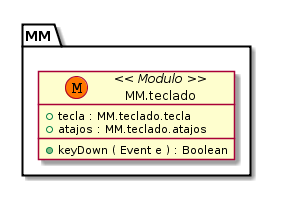
\includegraphics[width=0.4\linewidth]{imagenes/diagrama-clase-mm-teclado}
\caption{Clase MM.teclado}
\label{fig:diagrama-clase-mm-teclado}
\end{figure}

El sistema de control de teclado se encarga de recoger todos los eventos\footnote{Todos los eventos KeyDown del navegador.} de pulsación de teclas y revisar y calcular si se trata de un atajo registrado en el sistema y lanzar la función asociada a dicho atajo.

\begin{figure}[tbph]
\centering
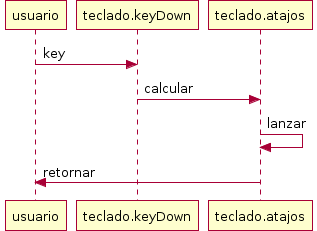
\includegraphics[width=0.4\linewidth]{imagenes/diagrama-seq-teclado}
\caption{Diagrama de secuencia teclado}
\label{fig:diagrama-seq-teclado}
\end{figure}

